\chapter{Introduction}

\hl{cite} \cite{ebner2008generalized}: using a solver for optimal instruction selection

A \gls{compiler}
  is a tool which
  converts from one representation
  to another---%
  usually, from a
  higher-level,
  human-readable representation
  to a lower-level,
  machine-readable representation.
A classic example
  is the clang compiler
  from the LLVM suite,
  which
  compiles programs written in 
  processor-independent C code
  into processor-specific
  machine code,
  which the hardware understands how
  to execute:
\begin{figure}[!h]
\centering
\begin{tikzpicture}
  \draw[inner sep = 5pt] (0,0) node [draw, thin] (c) \bgroup%
\begin{minipage}{10em}
\begin{minted}[fontsize=\small,baselinestretch=1]{c}
int square(int num) {
    return num * num;
}
\end{minted}
\end{minipage}
  \egroup;
  
\draw[inner sep = 5pt] (8.75,0) node [draw, thin] (asm) \bgroup%
\begin{minipage}{7em}
\begin{minted}[fontsize=\small,baselinestretch=1]{asm}
square:
 imul edi, edi
 mov eax, edi
 ret
\end{minted}
\end{minipage}
  \egroup;

\draw[inner sep = 5pt] (4.5,0) node [draw, thin] (compiler) {clang};

  \draw[->, very thick] (c) edge (compiler) (compiler) edge (asm);
\end{tikzpicture}
\end{figure}

\noindent
In this case,
  clang is generating code 
  for an x86 processor;
  we refer to 
  the platform
  which the compiler is compiling for
  as the \gls{target}.
Though compilers perform many target-agnostic
  transformations and optimizations
  (modifications of the high-level code
    which are useful regardless of the target),
  a compiler's fundamental purpose
  is to produce a program
  in the target's language.
For example,
  while clang has many optimizations
  it can perform
  before knowing what its target is,
  it eventually needs to produce x86
  assembly code
  such as in the example above.
We use the term
  \gls{compilerbackend}
  to refer to the target-specific portion
  of the compiler
  which implements this process.

Throughout this intro,
  we will use three different compilers
  as our running examples.
As we have already seen, we will
  consider the
  general-purpose C compiler
  clang
  as our ``gold standard'' example
  of a commonly-known
  and understood compiler.
However, we will also consider
  two compilers from more specialized
  domains,
  which will be key to
  \cref{part:glenside-and-3la}
  and
  \cref{part:lakeroad}
  of this dissertation,
  respectively.
First,
  the TVM compiler~\cite{tvm,chen2018tvm},
  which will be a main character
  of \cref{part:glenside-and-3la},
  is a compiler for deep learning
  programs
  which compiles code written in a
  high-level
  Python
  \gls{dsl}
  into optimized code
  for CPUs, GPUs,
  and custom accelerators.
\hl{ insert example?}
Second,
  the open-source \gls{hardwaresynthesis}
  tool Yosys
  is a compiler for hardware designs,
  and will be a focus of
  \cref{part:lakeroad}.
\hl{figure?}

\hl{instead of models then algos, algos then models.}
To implement the lowering
  from a high-level representation
  to target-specific code,
  compiler backends use a number of
  \textbf{algorithms}
  depending on the domain.
A key step in 
  compiling our
  example above
  is
  \textit{instruction selection:}
  deciding how to implement
  the various parts of the C program
  using actual instructions
  implemented in the hardware.
In the \texttt{square} function,
  clang must decide how to implement
  C's \texttt{*} operator---%
  in this case, using x86's
  \texttt{imul} instruction.
clang does this using
  an \textit{instruction selection}
  algorithm~\cite{llvminstructionselection}.
Steps akin to instruction selection
  exist in our other two compiler examples,
  as well.
TVM, for example, implements a step
  called 
  \textit{tensorization}~\cite{tvmtensorization}
  which maps high-level 
  machine learning kernels \hl{define}
  to target-specific implementations,
  including invocations
  of specialized hardware.
Similarly,
  a core step in hardware compilation
  for
  Yosys and other \hl{hardware synthesis tools}
  is \textit{technology mapping,}
  in which the tool determines
  how to implement the high-level
  hardware design
  using the hardware primtives
  available on the hardware
  platform.

Compiler backends 
  utilize \textbf{models} of hardware
  in the implementations 
  of their core algorithms.
% Whether or not they are apparent,
%   built into every compiler backend
%   are \textbf{models}
%   of the target platform.
These models come in all shapes
  and sizes.
For example,
  within clang, there is a list
  of the x86 architecture's
  instructions.
Here,
  we show the declaration of
  the integer multiplication
  instruction
  \texttt{imul},
  which clang used to implement
  the \texttt{square} function above:
  
\begin{figure}[H]
    \centering
%defm MUL : Mul<0xF7, "mul", MRM4r, MRM4m, mul>;
\begin{minted}[baselinestretch=1]{cpp}
defm IMUL : Mul<0xF7, "imul", MRM5r, MRM5m, null_frag>;
\end{minted}
\caption{
Declaration of x86's
  \texttt{imul}
  instruction in LLVM's x86 
  backend~\cite{llvmx86tablegen}.
}
    \label{fig:intro:llvm-tablegen}
\end{figure}

\noindent
clang's instruction selection algorithm
  uses
  this model of
  x86's instruction set
  to determine what instructions
  are available for selection.

Different models
  can capture very different things.
The deep learning compiler TVM,
  for example,
  declares 
  hundreds of different NVIDIA GPUs,
  including information
  about their internal capacities:


\begin{figure}[H]
    \centering
\begin{minted}[baselinestretch=1]{cpp}
TVM_REGISTER_CUDA_TAG("nvidia/nvidia-h100", "sm_90a", 49152, 65536)
    .with_config("l2_cache_size_bytes", Integer(52428800));
TVM_REGISTER_CUDA_TAG("nvidia/nvidia-a100", "sm_80", 49152, 65536)
    .with_config("l2_cache_size_bytes", Integer(41943040));
\end{minted}
\caption{
Declarations of NVIDIA GPUs
  within TVM~\cite{tvmgpudecls}.
}
    \label{fig:intro:tvm-gpu-decls}
\end{figure}


\noindent
These GPU declarations
  are a very different type of model
  from those shown in
  \cref{fig:intro:llvm-tablegen};
  instead of declaring instructions
  implemented by the hardware,
  these models capture
  capacity information.
\hl{tensorization}
However, similar to the model in 
  \cref{fig:intro:llvm-tablegen},
  these models of GPU hardware
  are used by TVM's GPU backend
  algorithms
  \hl{how?}
These examples serve to show
  that models are not only pervasive
  within compilers,
  but also that
  they come in many forms.
\hl{there is no way to build a compiler
  without encoding some kind 
  of model of the hardware;
  maybe this should go later, when we talk about implicit models?}

Lastly, for an example from Yosys,
  we look to its implementation of
  technology mapping.
This algoirthm
  is searching for a specific pattern 
  in the hardware design:


% Lastly, as an example from
%   yet another different domain,
%   this code snippet~\cite{yosysxilinxpmgen}
%   comes from
%   the open source hardware synthesis tool 
%   Yosys's~\cite{wolf2013yosys}
%   \texttt{pmgen} framework:

\begin{figure}[H]
    \centering
\begin{minted}[baselinestretch=1]{c}
subpattern in_dffe
arg argQ clock
code
  dff = nullptr;
  if (argQ.empty())
    reject;
  for (const auto &c : argQ.chunks()) {
    if (!c.wire)
      reject;
    ...
\end{minted}
    \caption{
Snippet of code
  from Yosys's pmgen framework~\cite{yosysxilinxpmgen}
  attempting to map hardware designs
  to specific hardware primitives.
    }
    \label{fig:intro:yosys-pmgen}
\end{figure}

% This code
%   captures a model of a specific hardware platform's functionality;
%   specifically, it checks whether
%   there is a \textit{D flip-flop}
%   (a specific hardware primitive)
%   on the input of a hardware module,
%   and folds it in to a larger module
%   if so
%   (which is omitted).

\noindent
Unlike the clang and TVM examples,
  which show declarative hardware models
  that are later used by algorithms,
  the above example is both algorithm
  \textit{and} model:
  encoded \textit{implicitly}
  within this algorithm
  is a model of the underlying hardware.
\hl{why are we talking about this?}

The current state-of-the-art
  when it comes to compiler algorithms
  using hardware models
  has many shortcomings:
  missed
  \cref{thesis:optimizations},
  \cref{thesis:correctness}
  issues,
  and 
  increased developer time
  (\cref{thesis:devtime})
  and effort.
We will now
  elaborate on each of these three topics.

\paragraph{\cref{thesis:optimizations}.}
If compilers rely on models
  of hardware
  when implementing optimizations,
  then, depending on how the model
  and the optimization is written,
  key optimizations can be left on the table.
Consider the snippet of Yosys code
  shown in
  \cref{fig:intro:yosys-pmgen}.
This snippet captures a specific optimization:
  utilizing an inbuilt feature of a hardware block,
  rather than adding additional hardware
  (i.e., another register) to solve the problem.
However,
  \hl{blah blah what could break?}
\hl{would be nice to show that automated methods have clearly shown
  to be superior when it comes to optimizing programs.
  STOKE, AutoTVM, synthesis in general, ML guided?}

\paragraph{\cref{thesis:correctness}.}
Second, compilers
  which rely on models of hardware
  can have hard-to-find bugs.
\hl{todo}

\paragraph{\cref{thesis:devtime}.}
And lastly,
  models of hardware
  built into compilers
  can oftentimes make compiler development
  more difficult.
This happens especially
  when models of hardware
  are \textit{implicit.}
For example, 
  compare the gcc example (\cref{fig:intro:gcc-imul})
  to the example from
  Yosys above (\cref{fig:intro:yosys-pmgen}).
You will notice that the
  gcc example is \textit{declarative:}
  it explicitly declares
  what the capabilities of the hardware are.
Meanwhile,
  the Yosys example is \textit{imperative:}
  rather than implicitly declaring
  the capabilities of the hardware,
  the capbailities of the hardware
  are \textit{implicitly} captured
  via a set of imperative instructions
  for matching a design
  to a hardware primitive.
Understanding implicit,
  imperative models
  is often more challenging
  than understanding explicit,
  declarative models.
Firstly, these models
  can be harder to find,
  as they are easier
  to embed implicitly into the compiler
  e.g.~within an optimization pass.
Secondly, as they are less explicit,
  it can be harder to reason about
  what they tell us about the underlying hardware.
% old version:
% In the worst case,
%   the model of a target
%   built into a compiler
%   can be \textit{implicit.}
% Unlike the example from gcc above,
%   in which the model \textit{explicitly}
%   describes the underlying hardware
%   without placing any undocumented
%   judgements upon it
%   (for example, how to perform a specific optimization),
%   \textit{implicit} models
%   are less declarative,
%   and implicitly encode more judgements.
% As an example
%   from a completely different domain,
%   this code snippet~\cite{yosysxilinxpmgen}
%   comes from
%   the open source hardware synthesis tool Yosys's
%   \texttt{pmgen} framework.
% This code
%   captures a model of a specific hardware platform's functionality.
% Specifically, it checks whether
%   there is a \textit{D flip-flop}
%   (a specific hardware primitive)
%   on the input of a hardware module,
%   and folds it in to a larger module
%   if so
%   (which is omitted):
% \begin{minted}[baselinestretch=1]{c}
% subpattern in_dffe
% arg argQ clock
% code
%   dff = nullptr;
%   if (argQ.empty())
%     reject;
%   for (const auto &c : argQ.chunks()) {
%     if (!c.wire)
%       reject;
%     ...
% \end{minted}
% We consider this model to be more \textit{implicit,}
%   as it encodes information
%   about the target
%   in an indirect way.
% Specifically, the above code
%   is making decisions
%   about how to use the underlying hardware platform,
%   and the only documentation for these decisions
%   are those left in code comments (omitted).
% In general, this model
%   is more \textit{imperative}
%   than the instruction model found within
%   gcc, which is more \textit{declarative}---%
%   the imperative nature gives more room for
%   implicit, undocumented decisions and preferences
%   to be encoded.
  

\hl{"all models are wrong, some are useful"

zach: not the case that implicit is worse; explicit can only express what fits in the model ie the DSL. implicit models have the flexibility of a more general language usually.

zach: why draw the fine line between explicit and implicit? First make points about limitations of models, then find a place to dig deeper later on.

implicit vs explicit flexibility: the power of negative expressiveness.

}

Thus, we have seen that
  existing approaches
  to building compilers
  using models of hardware
  can lead to missed optimization opportunities
  (\cref{thesis:optimizations}),
  issues with correctness
  (\cref{thesis:correctness}),
  and difficulty in compiler development
  (\cref{thesis:devtime}).

\hl{the strangeness of this first line is pointing out the fact taht we don't really want to be attacking models as a bad idea...we need a bit more nuance there. we need to make it clear we're pro model from the start.}
However,
  building compilers
  using models of hardware
  is still a good idea;
  in fact, in this dissertation,
  we will argue
  that existing approaches
  do not take the idea far enough.
We will specifically argue
  that compilers should be
  \textit{automatically} generated
  from formal models of hardware.
\hl{there's some spectrum here,
  of fully implicit models
  on the left,
  to automatic generation with explicit models
  on the right.}

\textbf{Explicit} models of hardware,
  on the other hand,
  are not only (1) pervasive (\cref{thesis:ubiquity}),
  but are also (2) prime for use with automated reasoning tools,
  in addition to (3) often being more correct.

\hl{a lot of this is true but for the hardware world. lots of stuff in the compiler world that's not good for automated tooling.

basically zach is saying, be cautious about applying this to general compilers i.e. llvm, gcc

domain specific accels + hardware, is the focus
}
  
\hl{Hardware models are pervasive:}
The reliance of modern compilers
  on \textit{implicit} models is truly odd, 
  given that
  explicit, formal models
  of the target hardware
  almost certainly exist
  in all cases.
In fact, nearly all hardware design
  \textit{begins} from the construction
  of these models
  at a high level of abstraction;
  the bulk of the hardware design process
  is building low-level implementations
  of the high-level specification,
  and verifying the implementation
  is equivalent.
Thus, \textbf{there is wealth
  of explicit, formal models of hardware
  which could be used
  instead of implicit models.}
\hl{examples of explicit hw models? alistair's work?
should probably go into a later paragraph}
\hl{maybe something about declarative programming being good?
a trend towards declarative programming?}

\hl{Hardware models are prime for use with automated tools:}
Furthermore, 
  there exist plenty of automated
  tools
  which deal with
  these formal models.
Oddly, though,
  many of these tools
  are concerned only with
  what happens \textit{after}
  compilation.
\hl{cite zach sisco latte, he says this directly}
That is, the formal models
  of hardware
  are used to check that 
  the compiled program is correct.
Why not instead
  just ensure
  that you can't compile an incorrect
  program?

\hl{The models are more correct:}
Lastly, and perhaps most importantly,
  these explicit models
  are perhaps \textit{more correct}
  than any implicit, handwritten models
  that could be written,
  as in many cases, these models
  are the \textit{ground truth.}

Furthermore, it is our position that
  \textbf{recent advances
  in programming languages
  make automated compiler construction
  feasible.}
The idea of automatically generating
  compiler backends is not new:
  previous work includes
  synthesizing instruction selectors%
  ~\cite{buchwald2018synthesizing,dias2010automatically,brandner2007compiler,daly2022synthesizing}
  and code generators~\cite{leupers1997retargetable,brandner2013automatic},
  among other work.
However, much of this work
  is a decade old, if not more,
  and does not benefit from
  advances in
  languages and type systems
  for hardware~\cite{durst2020type,nigam2023modular,nigam2020predictable},
  equational reasoning via equality saturation~\cite{tate2009equality,willsey2021egg},
  program synthesis~\cite{solar2008program,torlak2013growing},
  and machine learning for program generation~\cite{alon2019code2vec,austin2021program}.Furthermore, it is our position that
  \textbf{recent advances
  in programming languages
  make automated compiler construction
  feasible.}
The idea of automatically generating
  compiler backends is not new:
  previous work includes
  synthesizing instruction selectors%
  ~\cite{buchwald2018synthesizing,dias2010automatically,brandner2007compiler,daly2022synthesizing}
  and code generators~\cite{leupers1997retargetable,brandner2013automatic},
  among other work.
However, much of this work
  is a decade old, if not more,
  and does not benefit from
  advances in
  languages and type systems
  for hardware~\cite{durst2020type,nigam2023modular,nigam2020predictable},
  equational reasoning via equality saturation~\cite{tate2009equality,willsey2021egg},
  program synthesis~\cite{solar2008program,torlak2013growing},
  and machine learning for program generation~\cite{alon2019code2vec,austin2021program}.

Finally, this leads to my thesis statement:

\mdfsetup{
    frametitle={\colorbox{white}{\space{Thesis Statement}\space}},
    innertopmargin=10pt,
    frametitleaboveskip=-9,
    frametitlealignment=\center
    }
\begin{mdframed}
% Defined in toplevel imports-and-macros.tex
\mythesis
\end{mdframed}

In this dissertation,
  I present the case for
  automatically generating compiler backends
  from
  formal models of hardware.
I apply this technique
  to two separate domains:
  (1) compilation for
  domain-specific 
  deep learning accelerators,
  and
  (2) hardware compilation 
  (or \textit{synthesis})
  for Field-Programmable
  Gate Arrays (FPGAs).
In both of these cases,
  I show how
  automatically generating
  a portion of the compiler backend
  leads to increased correctness,
  greater extensibility,
  and more powerful automated optimization.

In the first part,
  I demonstrate
  how explicit,
  handwritten
  models of hardware,
  captured as
  \textit{rewrites,}
  can be used 
  to automatically implement
  ``instruction selection''
  for machine learning
  accelerators.

In the second part,
  I apply this thesis
  even more literally, by using
  formal models of hardware
  not written by us,
  but found in the wild,
  to build a compiler
  which automatically knows
  how to map designs
  to FPGAs.

The primary contributions of this dissertation
  are
\begin{itemize}

    \item blah
\end{itemize}


\hl{
TODO: people keep asking about the other direction;
  i.e. software generating hardware.
Have to explain why we're not doing that here.
}
  

\section{Argument Structure}

This section outlines the hierarchical
  argument
  of this dissertation.
At the top is the 
  thesis of the dissertation;
  everything else present
  in this dissertation
  is meant to prove this thesis.
The next level of bullets
  represent the arguments
  which directly support this thesis.
Following from this,
  each subsequent level of bullets
  represent the arguments
  which support the previous level of
  arguments.
We use the symbol ``$\Leftarrow$''
  to capture the fact that
  each sublevel of arguments
  taken together
  should imply their parent claim.
  
  

\textbf{Thesis:}
  Automatically generating
  compiler backends
  from formal models of hardware
  improves correctness,
  leads to emergent optimization,
  and increases extensibility.
\begin{itemize}[label=$\Leftarrow$]
 \item Generating the backend
      for a compiler for deep learning
      accelerators
      by modeling hardware
      as rewrite rules
      leads to
      emergent optimizations
      and more mapping opportunities.
 \begin{itemize}[label=$\Leftarrow$]
  \item blah
 \end{itemize}
 \item Generating an FPGA technology
   mapper
   using semantics
   automatically extracted
   from Verilog simulation models
   leads to greater correctness,
   completeness,
   and extensibility.
    \begin{itemize}
        \item The models already exist in the form of Verilog simulation models.
    \end{itemize}
\end{itemize}

\section{Roadmap}

How to read this thesis.

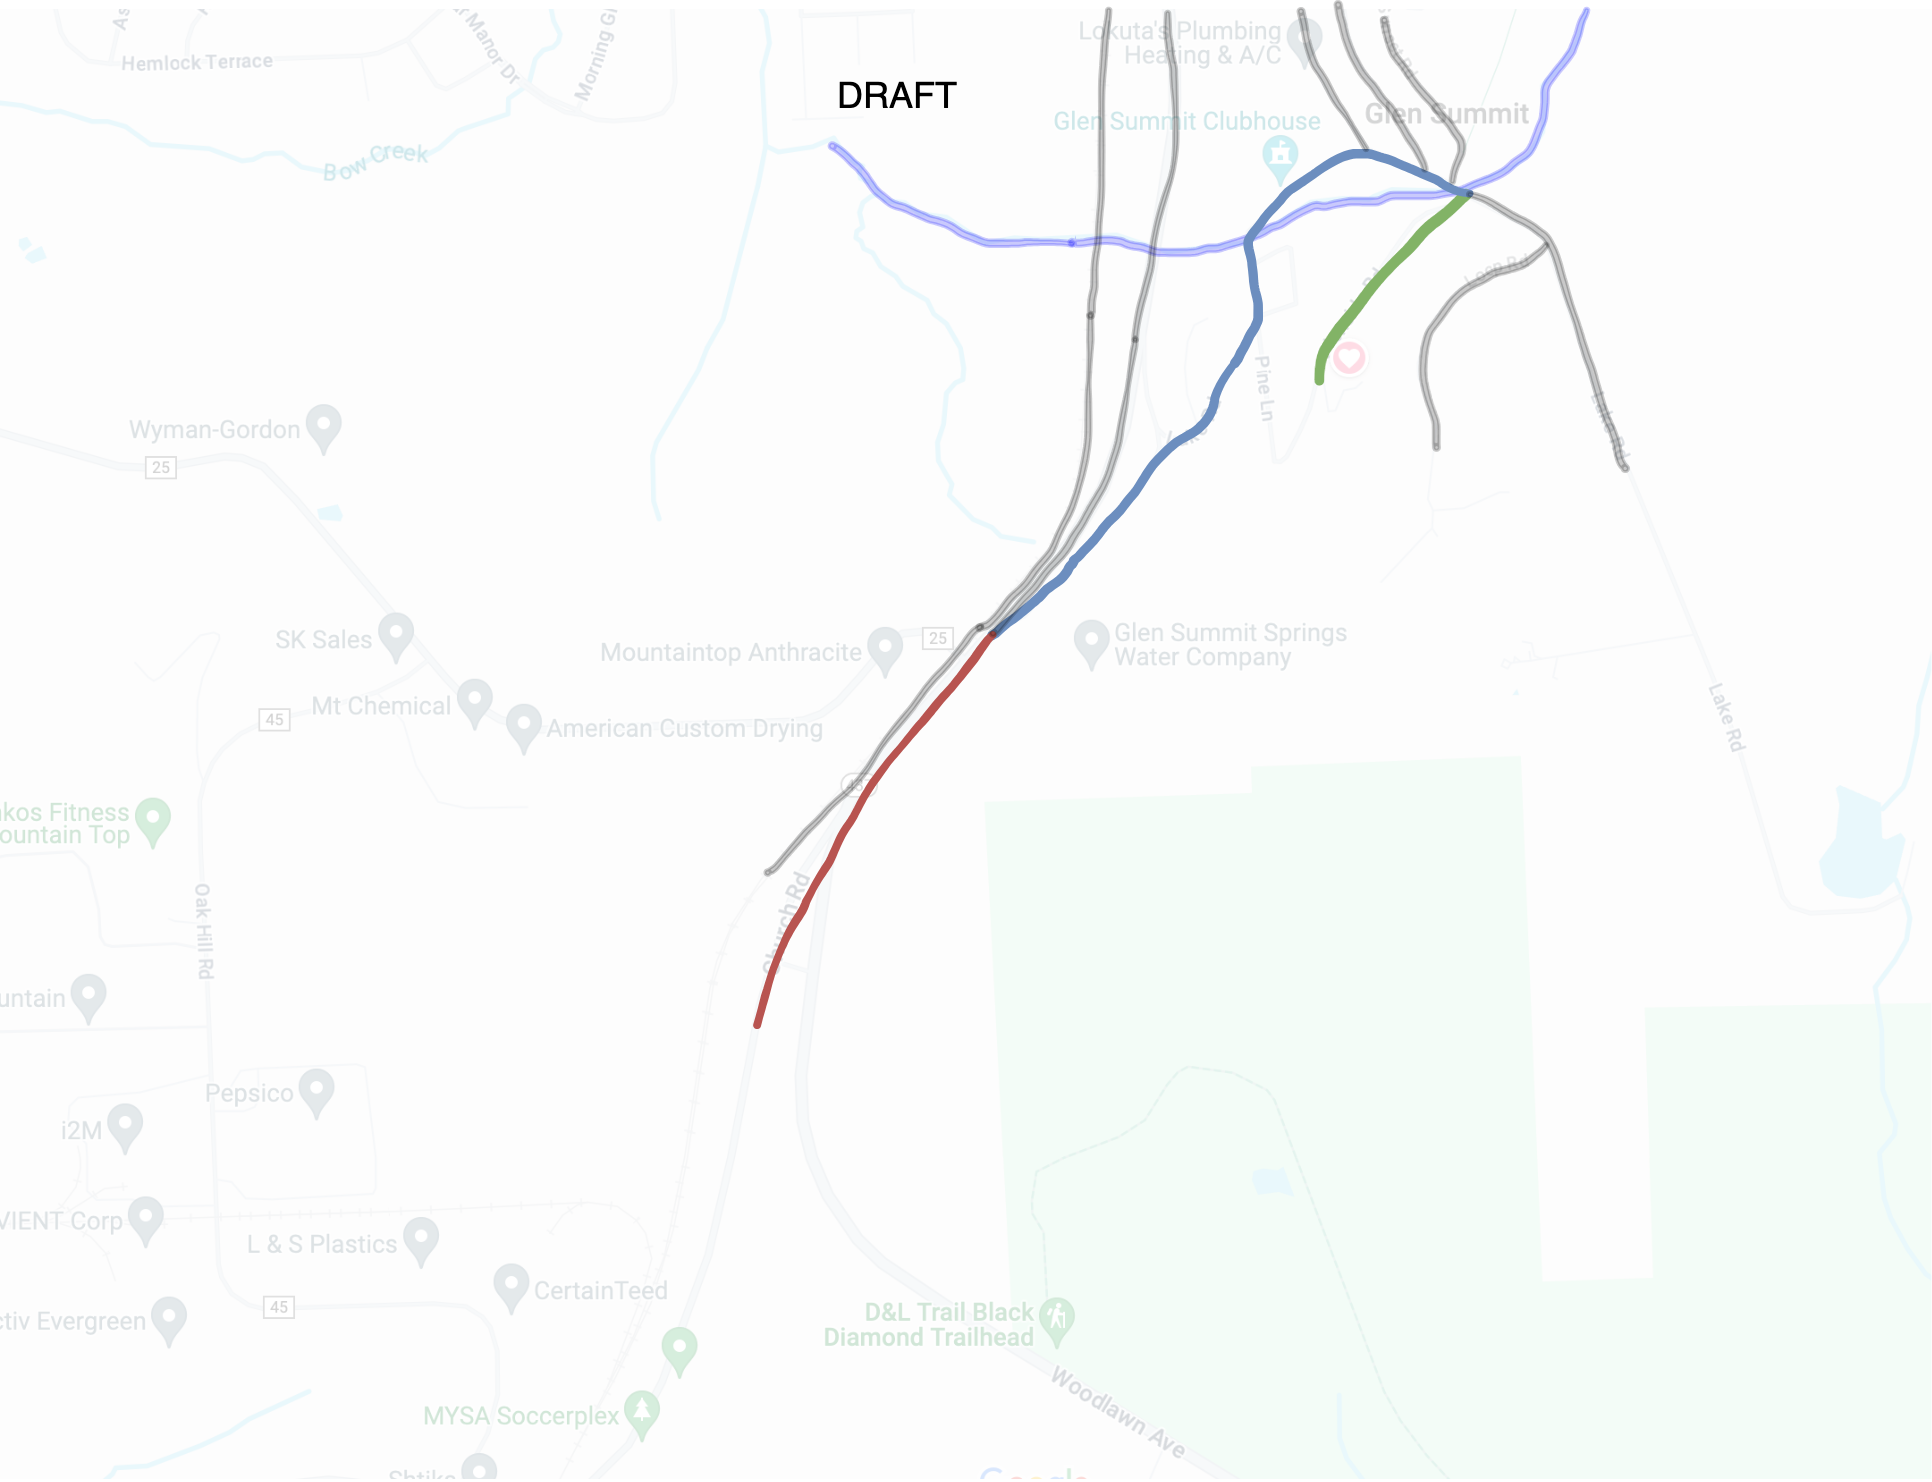
\includegraphics[width=\textwidth]{assets/street-diagram.drawio.png}